
La formación de un trombo en el interior de una arteria se denomina trombosis arterial. Esta formación de coágulos suele desencadenarse con la ruptura de una placa ateroesclerótica. Una placa ateroesclerótica es la manifestación principal de la aterosclerosis, que no es más que la acumulación de grasas, colesterol y otras sustancias dentro de las arterias y en sus paredes. La ruptura de estas placas es un acontecimiento muy trombogénico, al que se incorporan rápidamente las plaquetas.
La fibrina que contiene el coágulo aumenta lentamente a medida que el trombo se extiende por la luz arterial. Por ello, un trombo arterial contiene generalmente muchas plaquetas, aumenta rápidamente de tamaño y se ve expuesto a un flujo sanguíneo rápido.

Los trombos asociados a la arritmia se forman en entornos de bajo flujo y baja presión, por lo que los coágulos resultantes crecen lentamente y son ricos en fibrina. También se clasifican como trombos arteriales, aunque se asemejan más a los trombos de tipo venoso, cumpliendo así la tríada de Virchow para la trombogénesis:
        \begin{enumerate}
          \item Lesión endotelial.
          \item Lentitud del flujo o estasis sanguínea.
          \item Estados de hipercoagulabilidad.
         \end{enumerate}
\begin{figure}
    \centering
	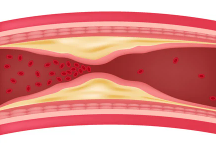
\includegraphics[width=0.50\textwidth]{figures/aterosclerosis.png}
	\caption{Arterosclerosis}
	\label{fig:example1}
  \end{figure}

\newpage Este tipo de coágulo sanguíneo puede causar ataques cardiacos bastante graves, si el taponamiento es en las arterias coronarias, o accidentes cerebrovasculares (en ocasiones irreversibles), si el taponamiento es en arterias cerebrales. La trombosis arterial es muy dañina para el organismo y, en general, mucho más grave y urgente que la trombosis venosa debido a la falta de oxígeno que provoca el taponamiento de las arterias en aquellos lugares donde están ubicadas. 
	
\section{Genes Asociados}
		La trombosis arterial se ve afectada por diversos genes. Este mapa nos muestra las interacciones entre los 25 genes que intervienen.\\
		
    \begin{figure}
        \centering
    	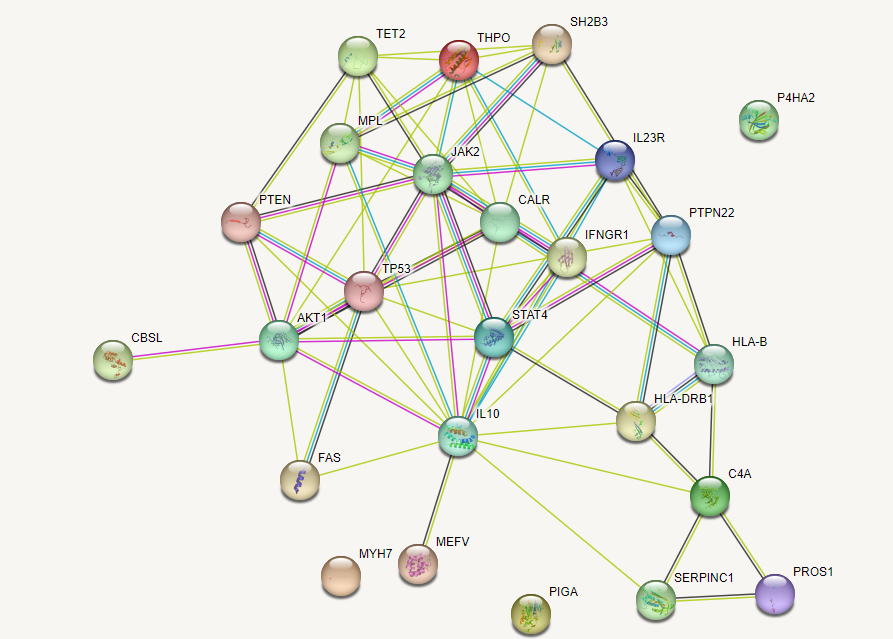
\includegraphics[width=0.50\textwidth]{figures/genes_asociados.png}
    	\caption{Genes asociados}
    	\label{fig:example2}
      \end{figure}
      
\subsection{STAT4 y JAK2}
          Como podemos ver, el gen STAT4 es relevante, ya que sirve como "punto de anclaje" para el bastantes de ellos, participando en multitud de interacciones entre ellos. Para explicar el funcionamiento de este gen es necesario nombrar a las quinasas Janus, en este caso, la JAK2.\\
		
		Las quinasas Janus están en el origen de diversas respuestas inmunológicas e inflamatorias y engloban 4 enzimas intracelulares de tipo tirosina-quinasa (JAK1, JAK2, JAK3 y TYK2 [tyrosine kinase-2]). En este caso, la que interviene en la trombosis es la JAK2 Estas enzimas están asociadas con la región membranosa intracelular de distintos receptores que convierten las señales extracelulares, mediadas por diversas citocinas u hormonas, en procesos intracelulares. La unión de una citocina al receptor causa su dimerización e induce la activación de las JAK asociadas. Cuando esto ocurre, las JAK fosforilan residuos específicos del dominio citoplasmático del receptor, donde se anclan los transductores de señales (STAT). Entonces se produce la fosforilación de los STAT que una vez activados se dimerizan y traslocan al núcleo, donde participan en la expresión de múltiples proteínas.\\
		
		Estas proteína es esencial para mediar las respuestas a la IL12 en los linfocitos, y regular la diferenciación de las células T helper, además de ser de suma importancia en la regulación del equilibrio entre ambas.  La deficiencia de Stat4 da lugar a una reducción de la aterosclerosis a través de la modulación de la función de las células B y del contenido de leucocitos en la aorta. Esta respuesta inmunológica hacia la anomalía de la arterosclerosis, provoca el aumento de leucocitos favoreciendo el taponamiento de glóbulos rojos. Es por ello, que las trombosis arteriales también son denominadas blancas.
	
